\section{Présentation de WooKey}\label{WooKey}

L'ANSSI développe depuis 2014 un projet de clé usb chiffrante sécurisée, le projet WooKey. Ce projet, open-source et open-hardware, s'inscrit dans le cadre d'une volonté croissante de la part de la communauté académique de sécuriser le protocole USB, notamment depuis la découverte et la publication de l'attaque BadUSB \footnote{L'exploitation d'une telle attaque rend possible, par exemple, la programmation de frappes sur un clavier afin d'injecter une charge dans une machine cible à partir d'un périphérique USB différent d'un clavier }

% mettre BadUSB-On accessories that turn evil en biblio

%The flexibility of the USB bus is also a weakness. Since various device classes can be plugged into the same connectors, a device can impersonate another one without any user action or notification. This can be performed by reprogramming the USB controller embedded in the device as it has been shown in the so-called BadUSB class of attacks [1]: many USB controller chips lack protections against such reprogramming.

%A common exploitation scenario is the HID Payload Attack: a malicious device is reprogrammed in order to act as a Human Interface Device (e.g. a keyboard) and perform custom keystrokes on the target machine to compromise it

L'objectif de WooKey est de fournir les fonctionnalités suivantes:
\begin{itemize}
	\item La protection des données des utilisateurs. L'ensemble des données sont chiffrées, ce qui permet d'assurer leur protection en confidentialité \footnote{la protection des données en intégrité n'est pas encore garantie (à confirmer)}
	\item L'utilisateur doit être présent lorsque les données sont déchiffrées (authentification forte)
	\item Le logiciel du périphérique doit pouvoir être mis à jour de manière robuste, les fichiers de mis à jour doivent en particulier être authentifiés et leur intégrité vérifiée avant toute mise à jour
	\item Les attaques logicielles doivent être prises en compte, afin de garantir qu'un attaquant ne puisse pas utiliser la surface d'attaque du logiciel (l'USB par exemple) pour obtenir un accès privilégié à la plateforme ainsi qu'un accès aux clés cryptographiques utilisées pour le chiffrement des données de l'utilisateur

\end{itemize}

Concrètement, la plateforme WooKey consiste en un micro-controleur 32 bits, de type STM32, se comportant comme un périphérique de stockage de masse. Les principales caractéristiques de sécurité de WooKey sont les suivantes:
\begin{itemize}
	\item Mise en oeuvre du concept de défense en profondeur,
	\item Logiciel de mise à jour sécurisé
	\item Double facteur d'authentification, utilisant une carte à puce et les principes de cryptographie les plus récents
	\item Une architecture logicielle modulaire, avec le cloisonnement des différents modules, présentée dans la figure suivante:
	\begin{itemize}
		\item Les modules TOKEN et PIN pour l'authentification double facteur,
		\item Le module CRYPTO pour le chiffrement des données transférées entre le périphérique et la machine hôte,
		\item Le module SDIO (Secure Digital Input/Output), pour le stockage des données chiffrées sur une carte SDIO,
		\item Le module USB, dans lequel le protocole USB 2.0 est mis en oeuvre. C'est dans ce module que se trouve la bibliothèque analysée dans le cadre de ce stage, décrite dans le paragraphe suivant.
	\end{itemize}
\end{itemize}

% 	\item Secure device software update: the device’s software should be robustly upgradable for system maintenance (e.g. security patches). Update files must be authenticated and integrity checked with no rollback to (possibly buggy) old versions. A software upgrade must be a voluntary and authenticated action. The firmware updates must be reliable with no possible platform bricking

% 	Firmware robustness against software attacks: the firmware should guarantee that an adversary attacking the exposed software surface (on the USB bus for instance) is not able to get a privileged access to the platform, and does not gain access to critical material such as sensitive cryptographic keys. Software attacks must be confined in unprivileged and isolated containers.

%WooKey platform: a custom STM32-based USB thumb drive with mass storage capabilities designed for user data encryption and protection, with a full-fledged set of in-depth security defenses. The device embeds a firmware with a secure DFU (Device Firmware Update) implementation using up-to-date cryptography as well as an external and extractable authentication token embedding a secure element.

\begin{figure}[!h]
\centering
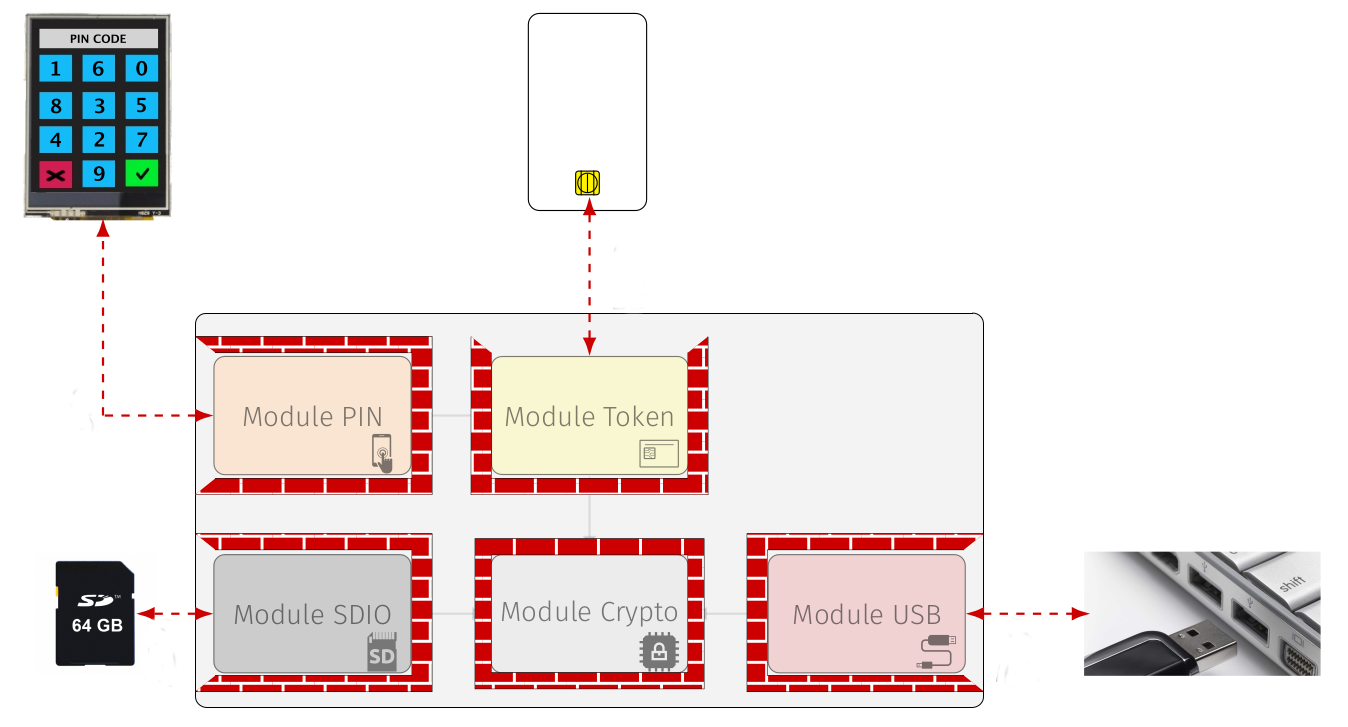
\includegraphics[width=16cm]{images/architecture_wookey.png}
\caption{Architecture logicielle de WooKey}
\label{Architecture logicielle de WooKey}
\end{figure}

\section{Présentation de la bibliothèque USBctrl}\label{USBctrl}

Avant de détailler la fonctionnement de la bibliothèque USBctrl analysée dans le cadre de ce stage, il est nécéssaire de présenter le protocole USB et ses spécifications.

\subsection{Généralités sur le protocole USB et spécifications de l'USB 2.0}

L'USB (Universal Serial Bus) est, comme son nom l'indique, un protocole de communication série entre entités. Plusieurs versions sont actuellement disponibles, de l'USB 1.0, la plus ancienne version, jusqu'à la version USB 4.0, la plus récente). WooKey peut actuellement fonctionner avec des versions USB inférieures ou égales à 2. Une des différences principales entre les différentes version est la vitesse de transfert des données entre un périphérique USB et une machine hôte (entre 1,5 Mbits/s et 480 Mbits/s dans le cadre de WooKey).
\newline
\noindent Du point de vue utilisateur, le bus USB se présente sous la forme d'une architecture étoilée et pyramidale, l'hôte se trouvant au centre du réseau, et les périphériques à l'extérieur. L'intérêt principal de ce bus est le fait qu'un grand nombre de périphériques (jusqu'à 126) peuvent être connectés simultanément au même hôte, et qu'à tout moment, il est possible de les débrancher et de les rebrancher sans redémarrer l'hôte. La figure suivante représente cet exemple d'architecture USB :

\begin{figure}[!h]
\centering
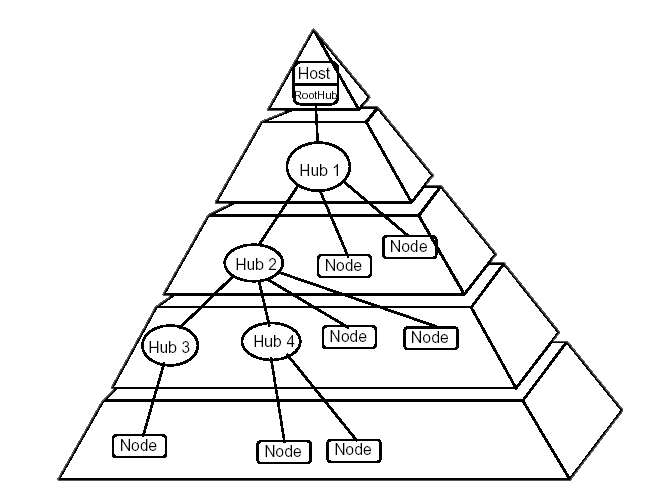
\includegraphics[width=16cm]{images/schema_etoile_USB.png}
\caption{Exemple d'architecture USB}
\label{Exemple d'architecture USB}
\end{figure}

Les périphériques USB peuvent être regroupés en classes et sous-classes USB, telles que, par exemple :
\begin{itemize}
	\item les claviers et les souris, faisant partie de la classe Humain Interface Device (HID),
	\item Les imprimantes,
	\item Le stockage de masse (MSC),
	\item Les lecteurs de cartes à puce.
\end{itemize}

Le protocole USB est enfin caractérisé par une machine à états, décrite dans les spécifications de l'USB 2.0 en référence XX. Cette machine à états est présentée dans la figure suivante :

\begin{figure}[!h]
\centering
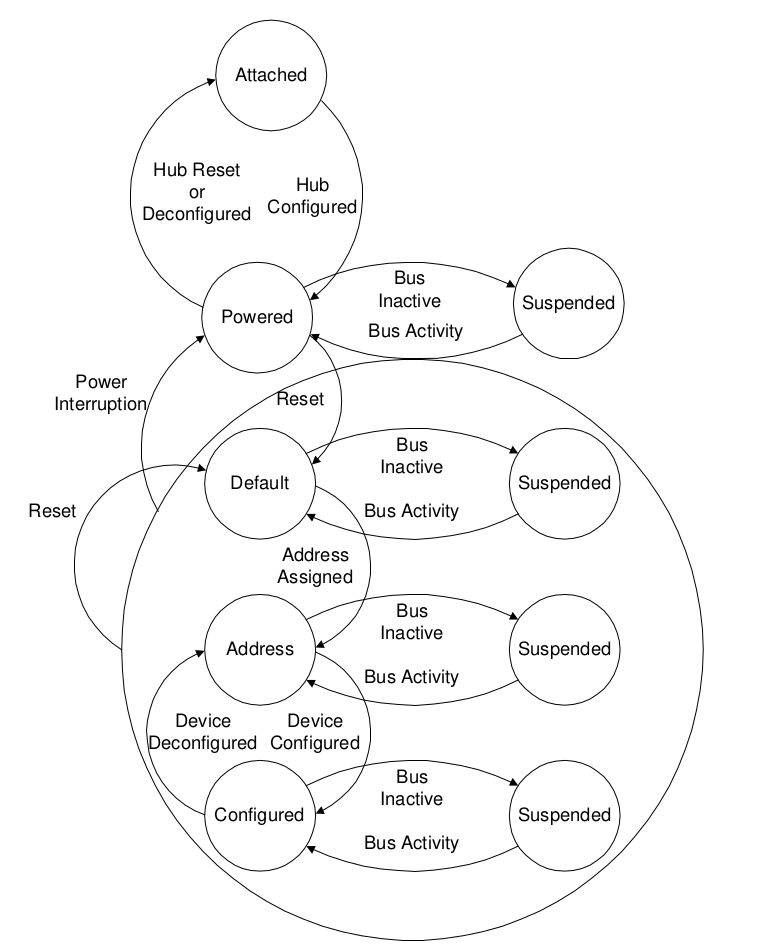
\includegraphics[width=16cm]{images/machine_etat_USB2.png}
\caption{Machine à états de l'USB 2.0}
\label{Machine à états de l'USB 2.0}
\end{figure}


\subsection{Rôle de la bibliothèque USBctrl dans le module USB de WooKey}

Chaque périphérique USB 2.0 nécessite la mise en place d'une structure de contrôle afin de pouvoir initialiser la communication avec l'hôte, négocier les propriétés du canal de communication USB mis en place avec l'hôte et déclarer les capacités du périphérique (vitesse de transfert des données par exemple).
\noindent C'est ce rôle que joue la bibliothèque USBctrl de WooKey. Elle permet par ailleurs de gérer la machine à états de l'USB 2.0, sans nécessiter d'actions complexes de la part des couches plus élevées du périphérique et, surtout, réalise l'abstraction du driver USB pour permettre une portabilité complète, quelque soit la classe USB ou le driver USB du périphérique.
\newline \noindent Le contrôle du protocole USB réalisé par la bibliothèque USBctrl est réalisé en manipulant des structures caractérisques du protocole USB:
\begin{itemize}
	\item les points de terminaison (ou endpoint), qui sont des canaux de communication à travers lesquels les données sont transmises. Chaque point de terminaison a un type (comment sont formattées les données) et une direction (depuis ou vers le périphérique). Les points de terminaison sont à sens unique, les données pouvant soient être reçues, soit être transmises à travers eux. La bibliothèque USBctrl utilise le point de terminaison 0, à travers duquel sont transmises les données permettant la configuration du protocole USB. D'autres points de terminaison peuvent être utilisés par la suite, afin d'échanger des données entre le périphérique et l'hôte, mais ces points sont utilisés par les couches applicatives du module USB et non par la bibliothèque USBctrl.
	\item les interfaces qui:
		\begin{itemize}
			\item définissent la classe et la sous-classe USB des couches applicatives en interface avec la bibliothèque USBctrl,
			\item déterminent si la configuration USB peut gérer une ou ou plusieurs interfaces (par exemple, un périphérique USB avec 2 ports USB peut avoir deux classes USB différentes qui peuvent être gérées au sein d'une même configuration),
			\item comprennent une liste de points de terminaison associés aux interfaces
		\end{itemize}
	\item le contexte USB, qui permet de gérer le point de terminaison de contrôle ainsi que les interfaces définies dans le périphérique. Ce contexte est caractérisé par un identifiant unique, par une adresse, par un état (au sens de la machine à état des spécifications de l'USB 2.0) et par le nombre des configurations USB du périphérique (un contexte peut avoir une ou plusieurs configurations différentes, et un périphérique USB peut avoir plusieurs contextes)
\end{itemize}

\noindent La figure suivante illustre le positionnement de la bibliothèque USBctrl dans la partie logicielle du module USB de WooKey. Cette figure permet notamment de visualiser les interfaces entre la bibliothèque USBctrl et les couches applicatives et entre la bibliothèque USBctrl et le driver USB.

\begin{figure}[!h]
\centering
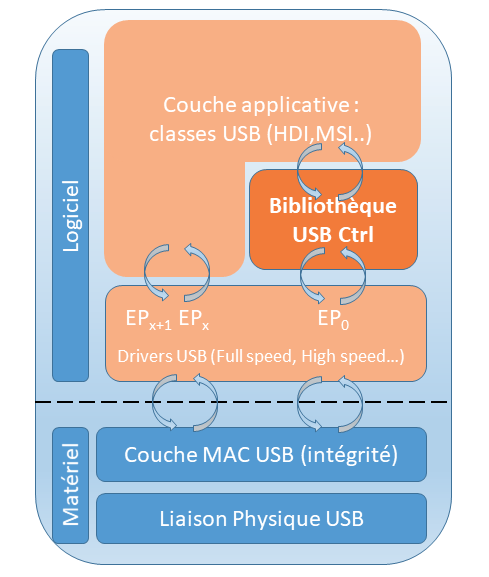
\includegraphics[width=16cm]{images/schema_usbctrl.png}
\caption{Schéma logiciel de la bibliothèque USBctrl}
\label{Schéma logiciel de la bibliothèque USBctrl}
\end{figure}

%A USB interface is the entity to which the host communicate through endpoints. A USB interface respects a given USB Class, subclass and protocol (for example, a mass-storage device is a USB MSC UMS Class, usually using SCSI reduced or transparent command set Subclass, and BBB (Mass-storage Bulk-Only) protocol. These three values are encoded on one byte and are standardized in the various USB Class specifications defined by the USB consortium. In USB devices, interfaces can be handled synchronously, or separately. This depends on interfaces constraints, which may be incompatible with each others. To do that, interfaces are associated to configurations. A configuration is a set of interface which is active at a given time. The host is responsible for requesting the list of valid configurations from the device, and can request configuration schedule, in order to switch from a set of interface(s) to another set of interface(s). The libUSBCtrl handle this.

% In the libUSBCtrl, a USB interface definition:
% • defines the USB interface class, subclass and protocol
% • specify if the interface must be in a dedicated configuration (this will create a new configuration dedicated to it)
% • provide an interface request handler, to support class requests, which are host requests targeting the USB inter-
% face instead of the USB device control plane
% • a class descriptor provider, if the class handle a class descriptor. If this provider is given, the class descriptor is
% added just after the interface descriptor in the configuration descriptor
% • a list of endpoints associated to the interface, as defined above

% The libUSBCtrl handle, for each USB hardware block declared, a USB context. This context, by default, only handle
% the USB default control pipe, which is common to any USB device.
% Then, interfaces is added to the context, and the context can be launched, by fully activating the device with the
% corresponding complete configuration.
% In the libUSBCtrl, interfaces are hold in a configuration structure. The context hold multiple configurations:

% The context:
% • is associated to a unique USB device associated to its device identifier and its device_t structure passed to the
% driver.
% • holds an address field, which is associated to the set_address standard request and is managed by the libUSBCtrl.
% • holds the number of different configurations, and the current configuration identifier
% • holds the state of the standard USB 2.0 state automaton






%Any USB 2.0 compliant device must implement a USB 2.0 control stack. THis control stack interacts with the xHCI USB stack of the host, in order to negociate the overall USB communication channel properties, speed, and to declare the device capacities.
%This control stack can be hard-coded or intelligent enough to support configuration and interface registration (i.e. multiple USB interface over USB standard control plane), defining an hybrid device, handling multiple USB classes and subclasses in the same time.
%This library is designed in order to:
	%support any USB class and handle the corresponding stack registration easily
	%handling correctly the USB stack automaton without requiring complex action from upper level classes
	%supports one or more interfaces in the same time
%This library is full software and does not directly handle the hardware USB device. This device is handled by a USB device driver with which this library interact in order to handle the control plane properly. Though, this library handle the driver choice and provide fast and efficient USB driver access abstraction to allow a complete portability of all USB classes implementations.




\section{Code source de la bibliothèque USBctrl}

\subsection{Description}

La bibliothèque USBctrl se compose de 5 fichiers, pour environ 2000 lignes de code, dans lequels sont implémentées une quarantaine de fonctions assurant les fonctionnalités de la bibliothèque présentées dans le chapitre précédent:
\begin{itemize}
	\item le fichier usbctrl.c, comprenant l'API de la bibliothèque USBctrl : déclaration et initialisation du contexte USB, déclaration des interfaces, des points de terminaison et démarrage du périphérique USB,
	\item Le fichier usbctrl\_state.c, comprenant les fonctions relatives à la gestion de la machine à états de l'USB 2.0,
	\item Le fichier usbctrl\_handlers.c, comprenant les fonctions relatives à la gestion de certains événements tels que la réception d'un signal de reset en provenance de l'hôte, ou la réception ou l'émission de données à travers l'endpoint de contrôle (EP0),
	\item Le fichier usbctrl\_descriptors.c, avec une seule fonction permettant de gérer la structure de données comprenant les caractéristiques des différentes configurations USB du périphérique,
	\item Le fichier usbctrl\_requests.c, dont les fonctions permettent de répondre aux requêtes émises par l'hôte à destination du périphériques USB (par exemple, demande d'information sur la configuration du périphérique \footnote{les différentes requètes auxquelles la bibliothèques doit pouvoir répondre sont définies dans les spécifications de l'USB 2.0})
\end{itemize}


% USB devices report their attributes using descriptors. A descriptor is a data structure with a defined format. Each descriptor begins with a byte-wide field that contains the total number of bytes in the descriptor followed by a byte-wide field that identifies the descriptor type. Using descriptors allows concise storage of the attributes of individual configurations because each configuration may reuse descriptors or portions of descriptors from other configurations that have the same characteristics. In this manner, the descriptors resemble individual data records in a relational database.
\noindent Comme expliqué dans le paragraphe précédent, la bibliothèque USBctrl réalise l'abstraction des drivers USB à travers des alias dans les différents fichiers de la bibliothèque. Cela permet à la bibliothèque de pouvoir être utilisée avec n'importe quel driver USB et de garantir sa portabilité, tout en évitant d'avoir une fonction contrôle pour chaque driver (contrainte de quantité de mémoire disponible dans le périphérique). Néanmoins, il est apparu très tôt dans le cadre de ce stage que la vérification formelle de la bibliothèque USBctrl, pour être précise, nécessitait de vérifier formellement les fonctions du driver appelées par la bibliothèque. Par conséquent, une partie du driver USB high speed présent dans WooKey a été analysé \footnote{ Deux drivers USB sont codés dans WooKey, le 2ème étant le driver full speed. Le driver high speed étant plus répandu, le choix s'est porté sur lui}
\newline
\noindent Le driver high speed se compose de 4 fichiers, pour environ 2000 lignes de code. Ses différentes fonctions permettent notamment :
\begin{itemize}
	\item De déclarer le contexte USB du driver USB et de le manipuler (initialisation, configuration...),
	\item De gérer le transfert de données entre le driver USB et l'hôte,
	\item De gérer les interruptions provenant de l'hôte,
	\item De lire ou d'écrire dans les registres mémoires du périphériques (adresses codées en dur, dépendantes du driver USB et du périphérique).
\end{itemize}

\subsection{Rappel sur le langage C}
% plutot dans une partie sur intérêt du stage : pourquoi la vérification formelle du code a du sens
La bibliothèque USBctrl analysée lors de ce stage est écrite en langage C. Ce langage de programmation est un langage de bas niveau, performant, qui permet aux programmeurs d'avoir un contrôle étendu sur leurs programmes, mais qui ne dispose pas des mécanismes de sécurité des langages de programmation plus récents comme Rust, en particulier pour la gestion de la mémoire. En effet, en C, la gestion de la mémoire est laissée à la charge du programmeur (allocation, désallocation, vérification de l'absence de buffer overflow..). Il est important de rappeler que la majeure partie des vulnérabilités logicielles découvertes ces dernières années sont dues à l'exploitation de buffer overflow.
\newline \noindent De plus, le standard du langage C ne spécifie pas l'ensemble des comportements du code, et donc certains restent indéfinis ou non spécifiés ce qui peut également mener à des RTE. A ce sujet, l'ANSSI a publié début 2020 un guide définissant un ensemble de règles, de recommandations et de bonnes pratiques dédiées aux développements sécurisés en langage C.

% mettre lien vers le site de l'ANSSI  + biblio


%The C programming language is a security nightmare. It is error-prone and unsafe, but, year after year, the conclusion remainsthe same: no credible alternative will replace C in a foreseeable future;especially in low-level developments or for constrained environments

%While many experienced programmers can write correct systems-level code, it’s clear that no matter the amount of mitigations put in place, it is near impossible to write memory-safe code using traditional systems-level programming languages at scale.

% pourquoi en C ? reflexion au début du projet pour le rust, qui présente des avantages en termes de sécurité, mais manque de stabilité au début du projet wookey. + compétences humaines (tous les programmeurs maîtrisaient le C + vérification formelle possible pour le langage C)

